%! Author = Vova
%! Date = 13.07.2021

% Preamble
\documentclass[11pt]{article}


% Packages
\usepackage{amsmath}
\usepackage{hyperref}
\usepackage{polyglossia}
\usepackage{graphicx}
\usepackage{babel,blindtext}
\usepackage{subfig}
\usepackage{iftex}

% Language and Font settings

% Kurale
% New Standard Old

\setdefaultlanguage{russian}
\setmainfont[Ligatures=TeX]{Kurale}
\newfontfamily\cyrillicfont{Kurale}

\title{Описание программной части робота-художника}
\author{Латыпов Владимир Витальевич}
\date{\today}

% Document
\begin{document}
    \maketitle
    \newpage


    \section{Формулировка задачи}

    Для того, чтобы робот-художник нарисовал что-либо, ему нужно предоставить данные в определённом формате, а именно — не набор пикселей,
    как требуется для показа на мониторе, а набор «мазков»: это связано с конструкцией самого робота.
    Мазки решено было представлять в виде кривых безье второго порядка (то есть квадратичных), к которым добавлены параметры «толщина» и «цвет».

    Но на вход подаются рисунки не в векторном, а в растровом формате.
    Найти такую комбинацию мазков, которая бы лучше всего соответствовала картине/изображению — задача нетривиальная, имеющая множество решений.

    Поэтому решено было использовать эвристические алгоритмы оптимизации:
    \href{https://en.wikipedia.org/wiki/Simulated_annealing}{Генетический алгоритм} и \href{https://en.wikipedia.org/wiki/Simulated_annealing}{Симуляция отжига}.

    Функцию ошибки необходимо задать таким образом, чтобы она отражала качество полученной комбинации мазков,
    причём в любой точке направление её уменьшения соответствовало направлению улучшения результата.
    Помимо напрашивающегося \href{https://en.wikipedia.org/wiki/Mean_squared_error}{MSE}, используемого

    \begin{equation}\label{eq:equation}
        MSE = \sum_{y = 0}^{y < height} { \sum_{x = 0}^{x < width} { \sum_{c \in  \left\{ r, g, b \right\} } { \left( {\overrightarrow {rendered_{x, y}}}_c - {\overrightarrow{original_{x, y}}}_c\right)^2 }}}
    \end{equation}


    \section {Алгоритмы оптимизации}\label{sec:opimization_algorithms}

    \subsection{Общий принцип ГА}\label{subsec:ga_general_principles}
    Идея работы Генетического алгоритма заимствована у природы.

    Точно также, как в ходе эволюции происходит появление оптимального организма для заданных условий,
    в ходе работы алгоритма ищется набор параметров функции, при котором фитнесс-функция максимальна.

    В природе тот, кто лучше приспособлен к окружающей среде, в большей степени получает доступ к размножению (с помощью различных механизмов),
    а при размножении новая особь наследует признаки каждого из родителей.

    Это позволяет именно лучшим чертам, по каким-либо причинам появившихся у особей, переходить в следующее поколение.
    Эти черты появляются через мутации — небольшие случайные изменения в геноме.

    Из принципа работы можно понять, что алгоритм \href{https://en.wikipedia.org/wiki/Heuristic_(computer_science)}{эвристический}: сложно доказать его сходимость или что-либо гарантировать с вероятностью 100\%.
    Зато \href{talgat.org/news/wp-content/uploads/2018/08/112.pdf}{исследования} показывают, что именно этот алгоритм даёт лучшие результаты для самых сложных функций.
    Далее мы увидим, какие меры предпринимаются, чтобы не дать алгоритму попасть в локальный минимум, не добравшись до глобального.

    \subsection{Термины}\label{subsec:ga_principles}
    Набор параметров представляется в виде \textit{«генома»} — некой структуры данных, содержащей информацию об этом наборе.
    \textit{Особь} — в контексте алгоритма будет использоваться в качестве синонима к геному.
    Геном состоит изх \textit{генов} — каждый из них содержит информацию о каком-либо признаке (в случае природы) или параметре (в случае ГА).

    В каждый момент времени алгоритм работает с \textit{популяцией} — набором геномов. Полный аналог популяции в природе.
    Мутация — как и в реальной жизни — небольшое случайное изменение генома без строго определённого направления.

    \subsection{Примерная последовательность действий ГА}\label{subsec:approx_ga_algo}
    В общих чертах работа ГА выглядит так:

    \underline{Инициализация}: Сгенерировать случайную популяцию, каждый ген каждого генома — в заданных пределах.
    Затем — повторять, пока не закончится заданное количество итераций или не будет достигнуто требуемое значение фитнесс-функции:
    \begin{enumerate}
        \item Посчитать фитнесс-функции для каждой из особей.
        Для большинства задач этот шаг занимает бОльшую часть времени исполнения, поэтому нужно оптимизировать именно его, в частности — параллелизовать, запуская независимые вычисления на нескольких потоках.
        \item Каким-то образом отобрать особи на скрещивание
        \item Произвести скрещивание, получив «отпрысков» — часть нового поколения
        \item Сформировать новое поколение, используя, возможно, в разных пропорциях, различные источники геномов, а именно:
                \begin{itemize}
                    \item Отпрысков, полученных на предыдущем шаге в результате скрещивания
                    \item Лучшие особи из прошлой популяции
                    \item Случайные особи —  чтобы не дать алгоритму сойтись раньше времени, попав в локальный минимум
                    \item Возможно, результаты скрещивания особей в числе больше 2
                \end{itemize}
        \item Произвести мутации в некоторых особях этого поколения (лучшие из мутаций внедрятся в популяцию на следующих итерациях)
        \item Если алгоритм подходит к концу, добавить лучший геном из предыдущего поколения (чтобы он не подвергся мутации)
    \end{enumerate}

    \subsection{Авторские Модификации  в ГА}\label{sec:my_modifications}

    Учитывая тот факт, что в большинстве задач, решаемых мною, бОльшая часть вычислительного времени ($>> 95\%$) используется для подсчёта функции ошибки, а не для маниппуляций с геномами
    (это подтверждается результатами профайлинга).
    То есть задача состоит в том, чтобы минимизировать количество подсчётов функции ошибки, даже ценой более долгой работы с геномами.

    Первое изменение — я решил отказаться от дискретного кодирования геномов.
    Для алгоритма по каждой переменной задан её диапазон.

    Традиционный подход — разделить диапазон на $2^N$ частей и кодировать номер части в геноме как битовую последовательность из $N$ бит.
    Для подсчёта функции ошибки этот номер перекодируется назад в соответствующую точку непрерывной величины.
    Мутацей в данном случае является изменение случайного количества каких-то битов этого номера.
    А скрещивание обычно происходит путём

    Предварительное тестирование показало бОльшую эффективность этого метода по сравнению с традиционным подходом, однако планируется провести тщательное тестирование (см. \ref{item:testing_system})

    Алгоритм реализован мной на языке C++, он хранится в GitHub репозитории \href{https://github.com/donRumata03/PowerfulGA}{https://github.com/donRumata03/PowerfulGA}.

    \section{Наблюдения}\label{sec:observations}

    \subsection{Неравенство зон}\label{subsec:inequality}
    Когда я заметил, что зоны, на которые Adobe Illustrator делит изображение, могут очень сильно отличаться в размере (отношение площадей может достигать 1000 раз),
    мне захотелось измерить это неравенство численно, чтобы при разработке нового алгоритма измерять его качество в том числе по этому параметру.

    Существует большое количество метрик, я решил выбрать основные из них:
    \begin{itemize}
        \item Индекс Джини (вместе с кумулятивным графиком распределения дохода (также известен как \href{https://en.wikipedia.org/wiki/Lorenz_curve}{кривая Лоренца}))
        \item Процент «дохода» 1\% самых богатых от общего «дохода» (В случае зон вместо дохода используется занимаемая площадь).
        \item Процент самых богатых, имеющих в сумме 50\% от общего дохода.
    \end{itemize}

    Индекс Джини рассчитывается как отношение площади между кривой Лоренца и «линией равенства» к площади под линией равенства.
    Иными словами, $G = \frac{A}{A + B}$ на этой схеме:

    \begin{figure}[h!]\label{fig:lorenz_curve}
        \centering
        \includegraphics[width=0.75\textwidth]{../images/typical_lorenz_curve.png}
        \caption{Типичная кривая Лоренца}
    \end{figure}
    Альтернативный способ посчитать коэффициент, использующийся в реализации:
    \begin{equation}
        G = \frac{\sum_{i=1}^{n}  \sum_{j=i+1}^{n}  \left| y_i - y_j \right|}{n \cdot \sum_{i=1}^{n} y_i}
    \end{equation}
    Чем индекс выше, тем большее неравенство наблюдается в стране.


    Результаты оказались впечатляющими:
    \begin{itemize}
        \item $Gini\_index \approx 76\%$
        \item 1\% крупнейших зон покрывают ≈ 18\% изображения
        \item 6.25\% зон покрывают половину изображения
    \end{itemize}

    Так выглядит кумулятивный график распределения площади:
    \begin{figure}[h!]\label{fig:cumulative_inequality_graph}
        \centering
        \includegraphics[width=0.75\textwidth]{../images/cumulative_inequality_graph.jpg}
        \caption{Кривая лоренца для зон}
    \end{figure}

    Нетрудно заметить, что ни в одной стране мира нет такого неравенства, как среди зон:

    \begin{figure}[h!]\label{fig:gini_index_world}
        \centering
        \includegraphics[width=0.75\textwidth]{../images/gini_index_world.jpg}
        \caption{Индекс Джини по странам мира}
    \end{figure}
    Даже в ЮАР индекс Джини составляет 57.8\%.


    \section{Дальнейшее развитие}\label{sec:todo}
    Несмотря на то, что программа уже работоспособна, есть ещё много идей и планов по её усовершенствованию:
    \begin{itemize}
        \item Внедрить \textit{быстрый пересчёт функции ошибки} — это улучшение давно напрашивается,
                но оно несколько теряет в эффективности из-за того, что в одной мутации в среднем изменяется
                не так мало мазков (однако это количество убывает со временем).
                В настоящий момент ведётся работа над внедрением.
        \item Разделение мазков по слоям.
                Нетрудно заметить, что при рисовании картин художники сначала проходятся по холсту черновыми мазками большого размера, а затем — прорабатывают детали.
                Таких уровней детализации зачастую бывает немало.

        Пример того, как художник (\href{https://www.youtube.com/watch?v=VaXHtai2alU}{https://www.youtube.com/watch?v=VaXHtai2alU}) рисует картину по слоям:


        \begin{figure}[h!]
            \centering
            \subfloat{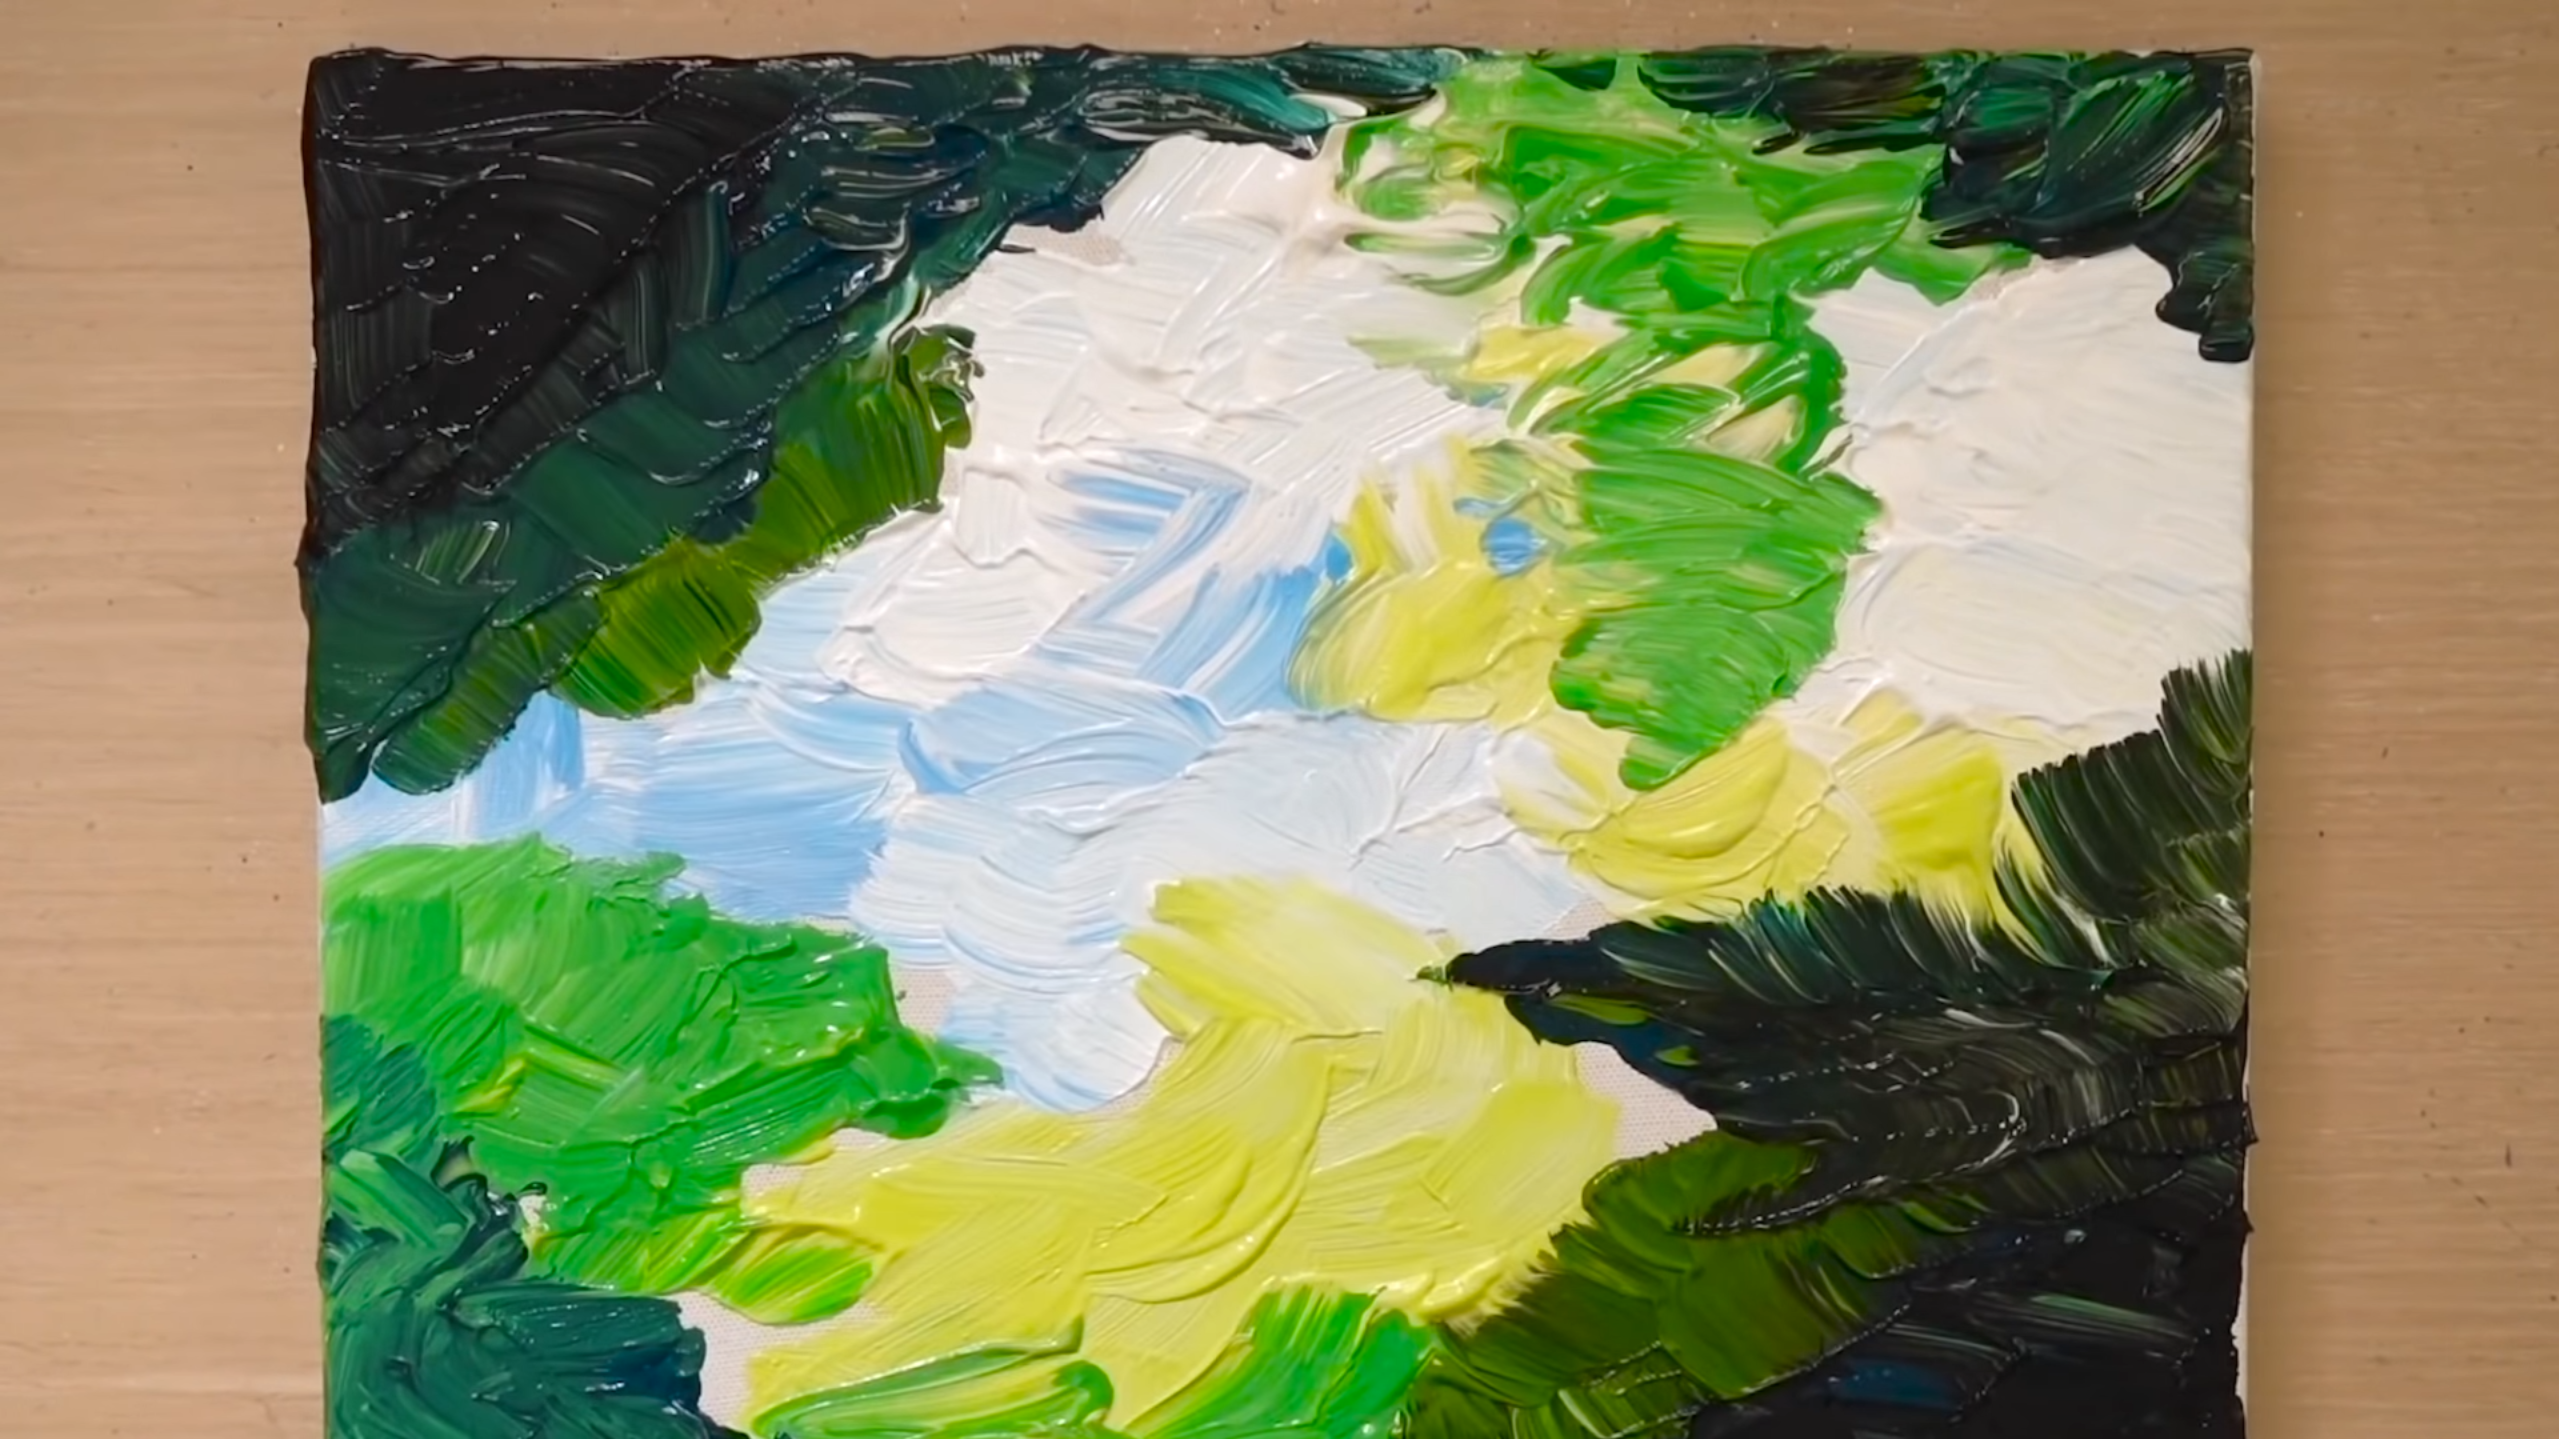
\includegraphics[width=0.24\textwidth]{../images/painting_example_layer_0.png}}
            \subfloat{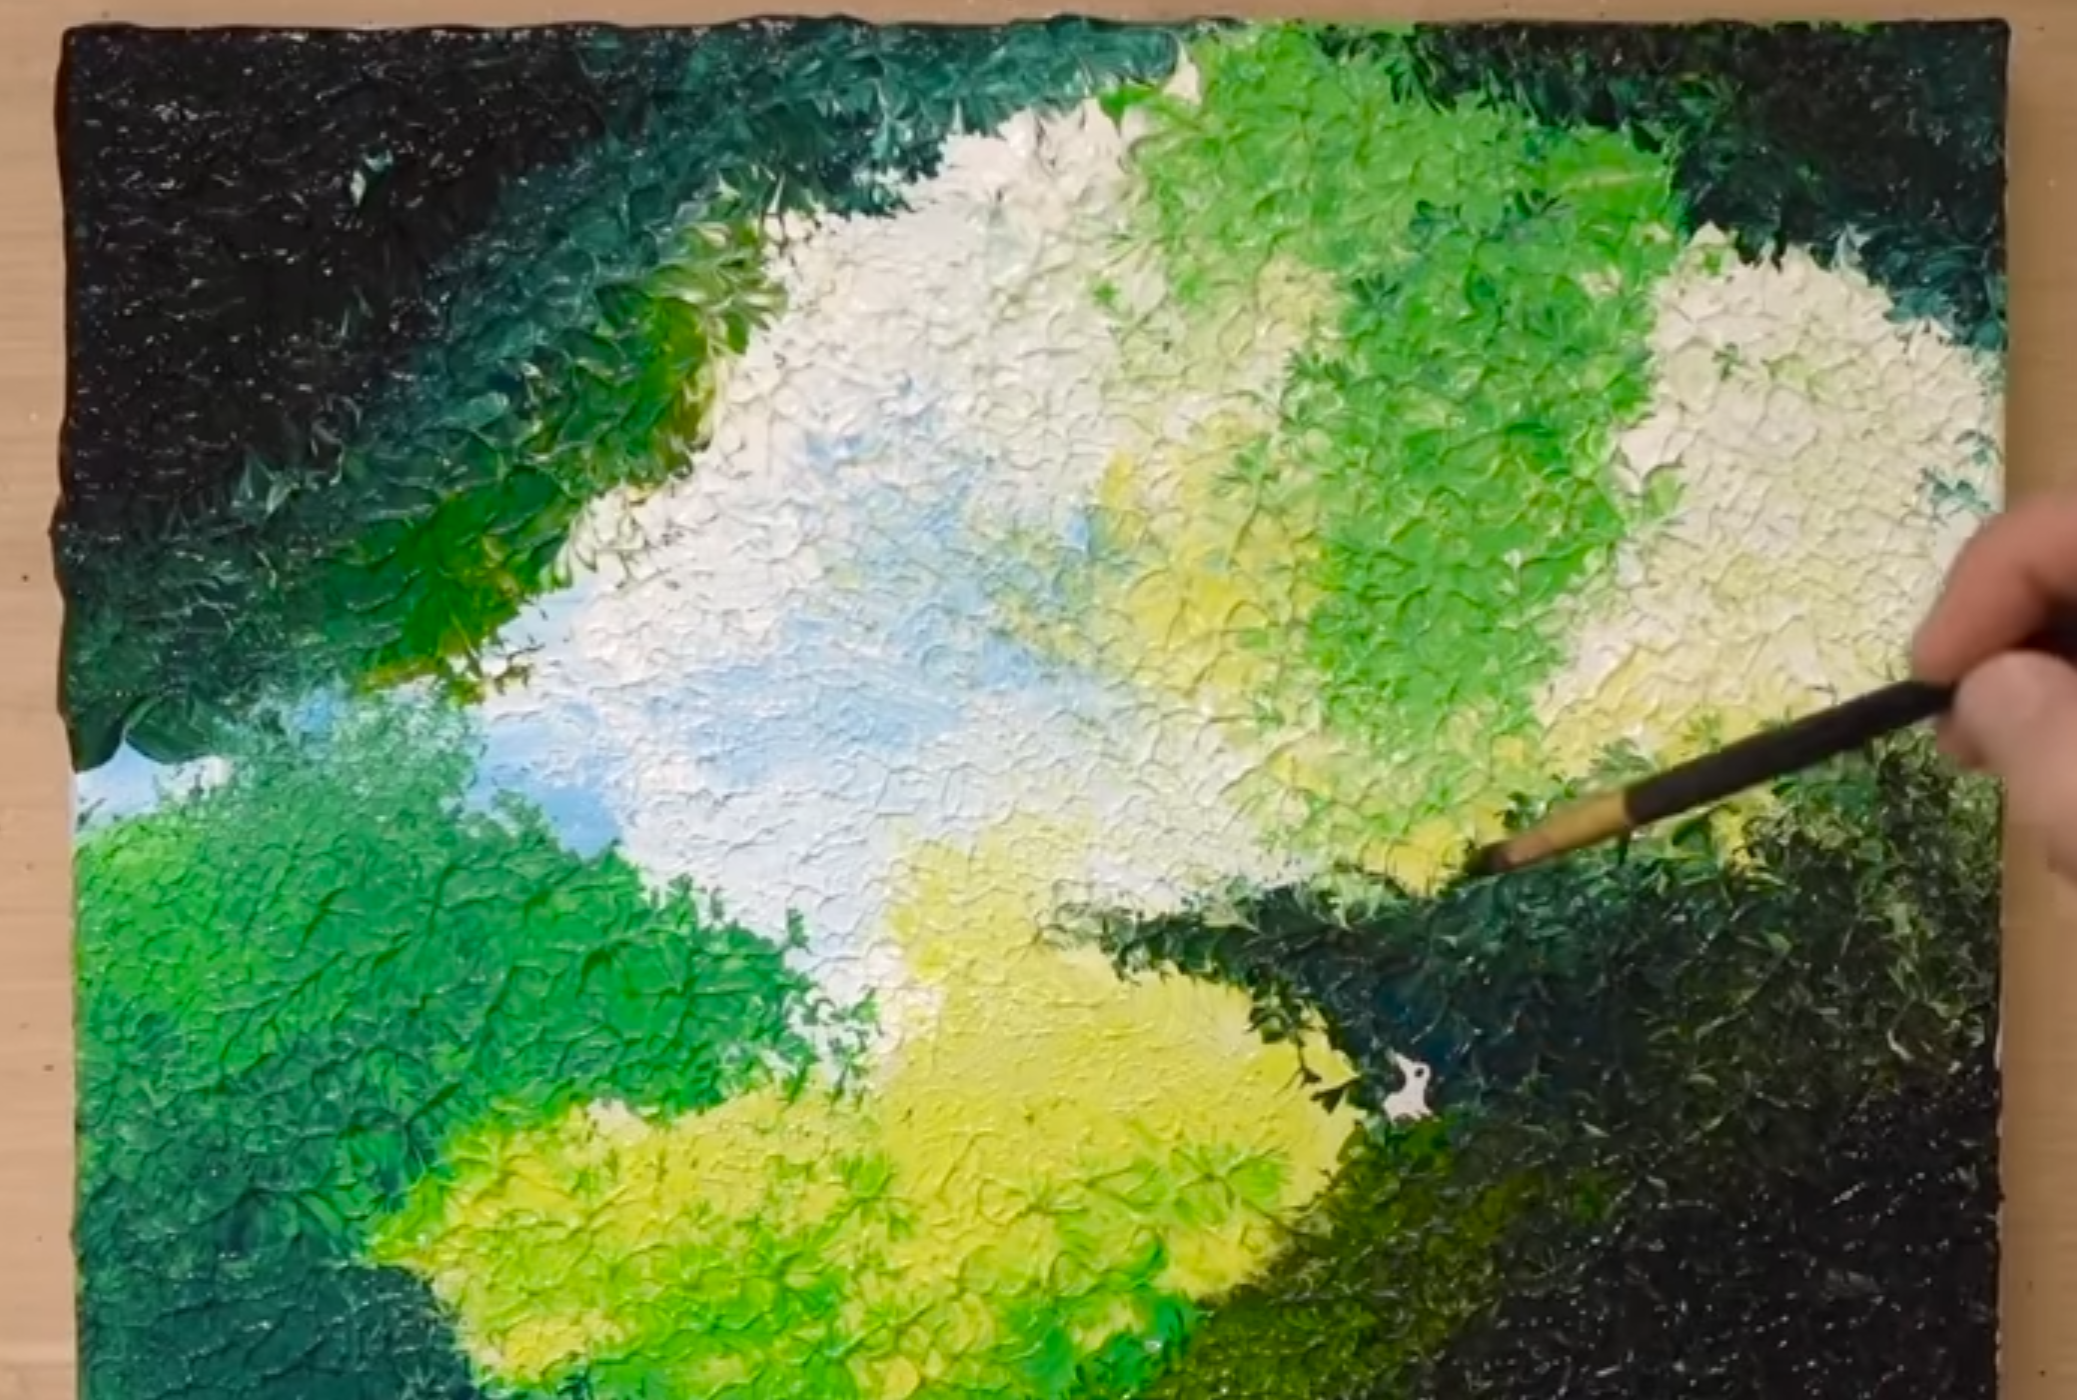
\includegraphics[width=0.24\textwidth]{../images/painting_example_layer_1.png}}
            \subfloat{\includegraphics[width=0.24\textwidth]{../images/painting_example_layer_2.png}}
            \subfloat{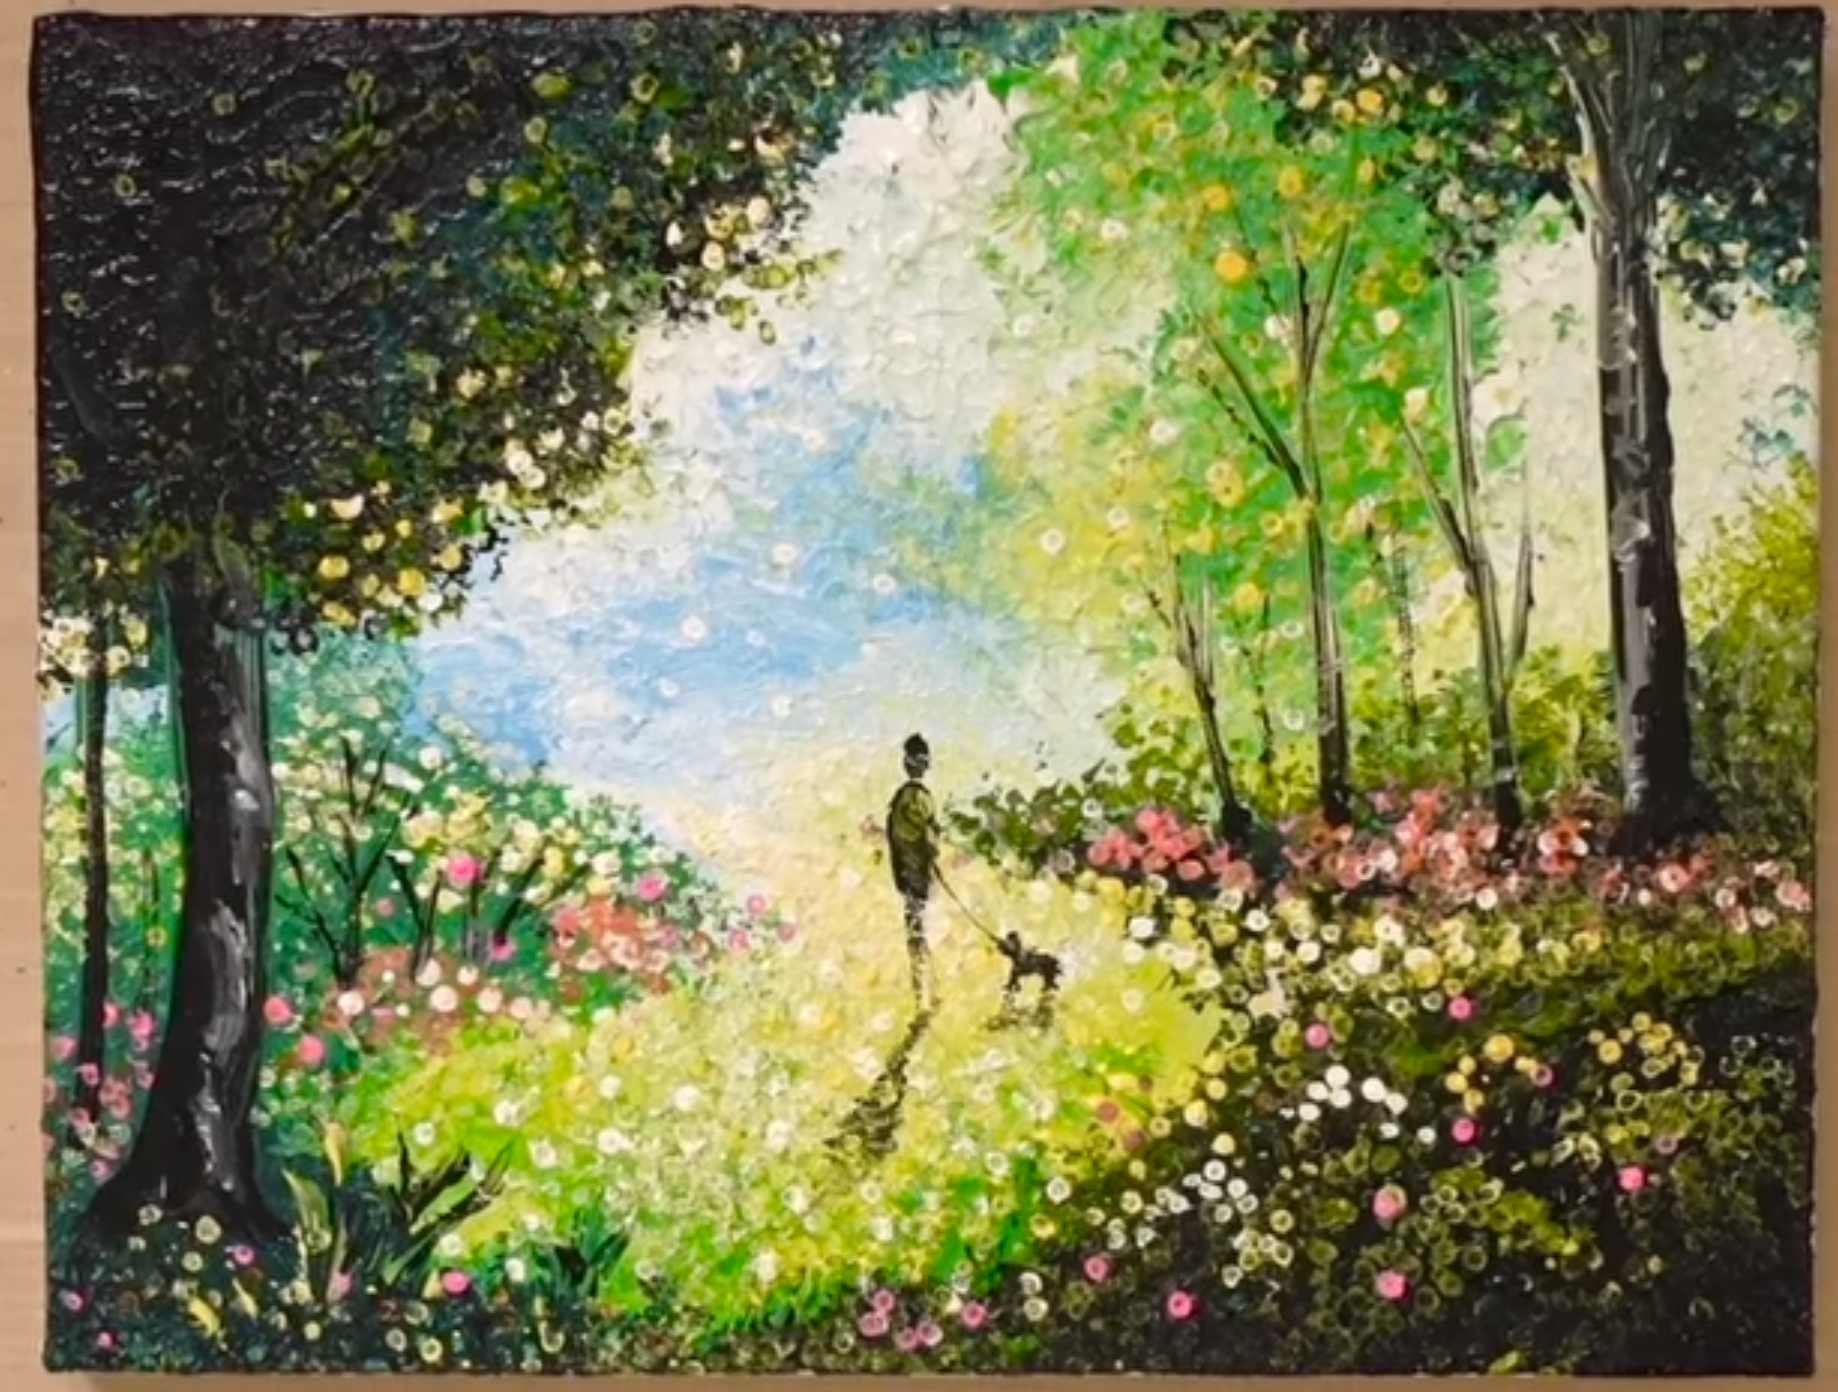
\includegraphics[width=0.24\textwidth]{../images/painting_example_layer_3.png}}
            \caption{ Фон | Рельеф фона | Детализация заднего плана | Основные объекты}
            \label{fig:layered_painting}
        \end{figure}


                Поэтому стоит попробовать сначала заполнять картинку толстыми, грубыми мазками
                (то есть просто с большей шириной, а в реальной жизни это будет отражаться в большем размере кисти и в более сильном нажатии).
        \item Добавить использование локальных методов оптимизации.
                Такие методы, как \textbf\textit{{градиентный спуск}} и \textbf\textit{{метод Ньютона}} позволяют достичь гораздо большей скорости сходимости
                (в случае метода ньютона — сходимость \href{http://w.ict.nsc.ru/books/textbooks/akhmerov/mo_unicode/4.html}{квадратичная}),
                но требуют умения посчитать градиент функции ошибки в любой точке, а также вектор вторых производных по каждому из аргументов.

                Сами алгоритмы реализованы и находятся в \href{https://github.com/donRumata03/PowerfulGA/blob/master/other_optimization/local_optimization.cpp}{этой папке}.
                Предусмотрена опция подсчёта первой и вторых производных через подстановку близких значений параметров:

                \begin{equation}
                    f'(x_0) \approx \frac{f(x_0 + \Delta x) - f(x_0)}{\Delta x}
                \end{equation}

                Однако в случае с мазками при маленьких изменениях параметров функция ошибки остаётся неизменной, так как это приводит к такому же набору закрашенных пикселей.
                Соответственно, нужно либо радикально увеличивать разрешение изображения, либо использовать аналитические методы.
                То есть нужно математически посчитать изменение функции ошибки при бесконечно малом изменении из параметров функции.

        \item \label{item:testing_system} Организовать систему тестирования различных алгоритмов на различных функциях.
        Звучит как нечто весьма простое, но реальность сложнее, чем кажется.
        Напрашивающийся вариант — дать каждому алгоритму заданное количество вычислений функции ошибки и сравнить, какой результат они получат.

        Однако функция ошибки нелинейная, поэтому сложно будет понять,
        насколько сильному различию в качестве алгоритма соответствует полученная численная разница в результатах.

        Целесообразно сравнивать количество итераций, требующееся алгоритмам для получения заданного результата.
        Но и тут не всё так просто: нельзя просто запустить алгоритмы на неограниченное количество итераций
        и ждать дотижения нужного значения функции,
        так как во многих из них (как минимум — в моей модификации ГА) то,
        как будет проведена каждая отдельная итерация, сильно зависит от процента выполнения на момент её прохождения:
        происходит планирование,  использующее информацию о максимальном количестве итераций.


        Поэтому нет никакого другого выхода, кроме того, чтобы запускать этот алгоритм с рахым количеством итераций и смотреть, когда он в среднем будет доходить до заданного порога.
        Это необходимо автоматизировать.
        В идеальном случае для поиска порога можно было бы использовать бинарный поиск, но в реальности (с поправкой на шум) имеет смысл использовать эвристическую модификацию н-арного поиска (объяснить!).
        Для полной оценки планируется построить график достаточного количества итераций от nребуемого значения функции в интересующей нас зоне.

        \item Улучшить алгоритм поиска цветов и разделения на зоны.

                Сейчас для разделения изображения на зоны используется Adobe Illustrator.
                По заданному количеству цветов (и, следовательно, уровню детализации) он разделяет изображение на зоны,
                присваивая каждой какой-то из цветов палитры так, чтобы он хорошо .
                Сама палитра тоже формируется в ходе работы алгоритма.

                Скорее всего, для этого используется один из популярных алгоритмов, описанных \href{https://en.wikipedia.org/wiki/Color_quantization}{здесь}, или некая проприетарная их вариация.
                Зоны, на которые происходит деление, описываются частями плоскости, ограниченными кривыми безье — «path»  формате $svg$.
                Несмотря на то что формально алгоритм выполняет свою работу, большое количество зон имеет очень продолговатую форму,
                а также наблюдается неимоверный разброс в размерах между разными зонами (см. ):
                всё это уменьшает эффективность процесса.





    \end{itemize}

\end{document}